
\chapter{Results} \label{ch:results}
This chapter aims to explore the operational boundaries of the chemical components in a Petri dish environment, focusing on the size limitations of the coincidence detector and the light sensitivity of a chemical diode.
A coincidence detector is crucial in the design of chemical circuits because it allows for an implementation of AND gates,
which are important for computing. This detector is illustrated in Figure \ref{fig:and-gate} and it works by having two waves come together from left and right and if they meet, they form a new wave that passes through the detector at the bottom.

The main objectives of the experiments are to find out the bounds and limitations of different chemical components in order to determine the feasibility of using them in a real-world environment.

\section{Creating a Coincidence Detector In Simulation} \label{chap:creating-detector}
The project aims to explore the mapping between the size of the computer in the simulation and the size of the computer in real life
according to Goal 1 in Section \ref{sec:goals-lit-review}. This cannot happen if there is no computer to begin with, so the first step is to create a computer in the simulation.
A whole computer would be cumbersome to create, so we start with creating a Coincidance Detector, also known as an AND gate, as it is one of the simplest computations that can be created in chemistry

Developing the AND gate posed a significant challenge as it is highly dependent on specific geometric configurations for proper operation. 
While it is acknowledged that such a coincidence detector is feasible, the focus of our investigation is on the stability of such simulations in response to environmental changes and the practicality of implementing them in a real environment.
Although we acknowledge that building this in a simulation is possible, the focus of this paper is to determine the stability of the simulation in response to environmental changes and the practicality of implementing them in a real environment. 


\subsection{Unsuccessful Detector}\label{unsuccessful-detector}
\begin{figure}
    \centering
    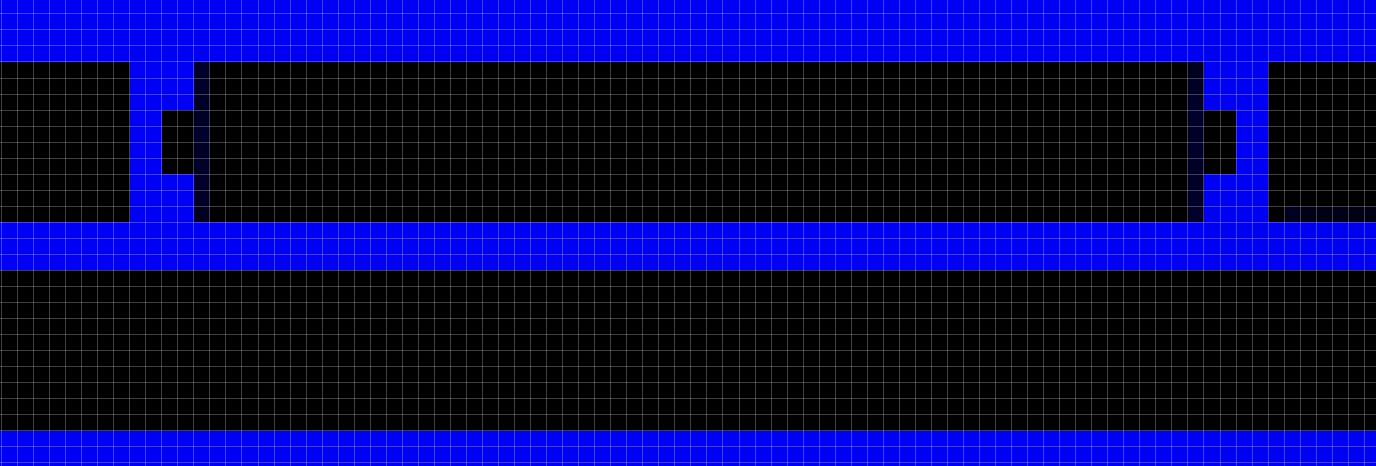
\includegraphics[width=0.75\linewidth]{image7.png}
    \caption{Initial Coincidence Detector Configuration}
    \label{fig:unsuccessful-config-and-gate}
\end{figure}
\begin{table}[h]
\centering
\begin{tabular}{|c|c|c|c|c|}
\hline
Width & Gap=1px & Gap=2px & Gap=3px & Gap=4px \\ \hline
w=1px & NP & NP & NP & NP \\ \hline
w=2px & NP & NP & NP & NP \\ \hline
w=3px & AP & NP & NP & NP \\ \hline
w=4px & AP & AP & NP & NP \\ \hline
w=5px & AP & AP & NP & NP \\ \hline
w=6px & AP & AP & NP & NP \\ \hline
w=7px & AP & AP & NP & NP \\ \hline
w=8px & AP & AP & NP & NP \\ \hline
w=9px & AP & AP & NP & NP \\ \hline
w=11px & AP & AP & NP & NP \\ \hline
w=12px & AP & AP & NP & NP \\ \hline
w=13px & AP & AP & NP & NP \\ \hline
\end{tabular}
\caption{Results of the experiment showing the relationship between conductor width and gap size.}
\label{table:experiment-results}
\end{table}
In our investigation, we focus on three controllable variables: 
\begin{itemize}
    \item the width of the conductor
    \item its length before the gap.
\end{itemize}
The detector configuration is shown in Figure \ref{fig:unsuccessful-config-and-gate}.
The primary question we seek to answer is how the width of the conductor influences the functionality of the gates. Specifically, our experiment aims to identify an optimal conductor width that enables the "if" gate to function correctly. This gate's operation relies on two conductors positioned closely, requiring a precise amount of force to facilitate signal transmission from one to the other. This force is generated by the collision of two waves. However, current configurations fail due to the conductors being excessively proximate.

For the purposes of this experiment, we define three outcomes based on the interaction between the waves and the conductors:
- Always pass (AP): The signal always passes through the gap.
- Never pass (NP): The signal never passes through the gap.
- Collision pass (CP): The signal passes through the gap only upon collision of waves.

The CP outcome is of particular interest as it represents the desired state for computational functionality.

Initial tests did not yield CP outcomes, suggesting a potential discrepancy in the values of $\phi_{\text{active}}$ versus $\phi_{\text{passive}}$. Adjusting $\phi_{\text{active}}$ to a more aggressive value of 0.035f resulted in CP outcomes for every gap of 3px, marking a significant deviation from the default value of 0.054 proposed in prior literature. This finding prompts further investigation into the range of values between 0.035 and 0.054 to identify a flexible operational window. 

A successful configuration identified involves a long charge, a gap of 3px, and a $\phi_{\text{active}}$ value of 0.035. Further exploration is required to determine a viable configuration for a gap of 2px.

Additionally, our observations reveal notable differences in wave behavior depending on orientation; specifically, vertical wave propagation exhibits distinct properties compared to horizontal propagation. A particularly intriguing observation is that waves originating off-center tend to accelerate asymmetrically, favoring one direction over the other, and resulting in a higher likelihood of collision.

\subsection{Successful Detector}

Section \ref{unsuccessful-detector} led to the conclusion that there must be more parameters in play that prevent the detector from functioning, and it was later found that the height of the diode pin on the active medium of the coincidence detector. 
Following this, it was discovered that by setting the pins higher or lower, we change from where the wave approaches the detector medium, allowing for a finer adjustment of the opration. This created the first successful detector, seen in Figure \ref{fig:first-successful-detector}.

\begin{figure}
    \centering
    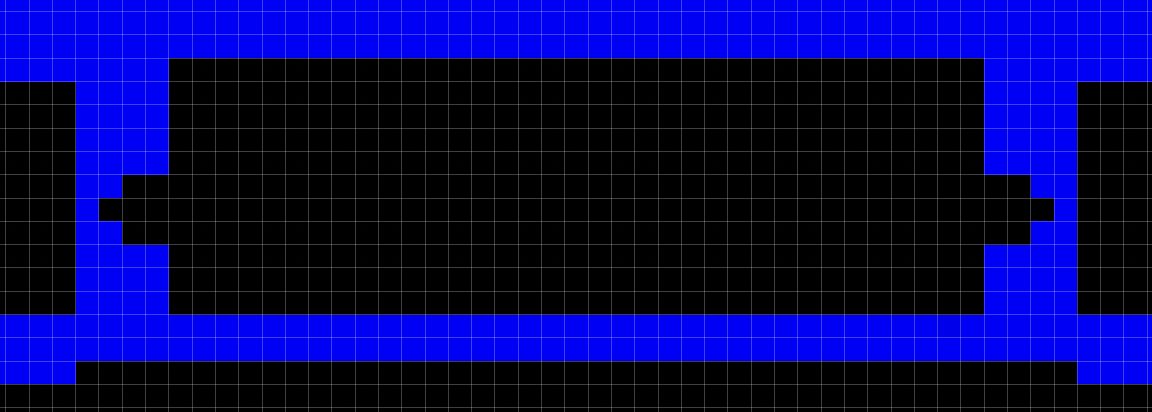
\includegraphics[width=0.75\linewidth]{image9.png}
    \caption{First Successful Coincidence Detector}
    \label{fig:first-successful-detector}
\end{figure}


Normally the wave also depends on where it is coming from, but we can ignore that in our case because we are using diodes at entry of the detector medium. Diodes add a new entry point for the incoming wave, so the incoming direction does not really matter. 

There is still a small problem with this design where if two waves meet around the centre, none of them gets enough momentum to develop fully and they do not have enough concentration to diffuse into the result substrate, this can be solved by increasing the length of the detector medium to allow for both waves to form, so later designs have a longer detector medium, like in Figure \ref{fig:and-gate}

The length of the coincidence detector depends on two factors:
\begin{enumerate}
    \item The minimum distance apart they need to be from each other while still allowing for the waves to form inside the detector.
    \item The minimum distance apart they have to be, so that the centre is still usable for collusion.
\end{enumerate}

This will be used in Section \ref{sec:mapping-simulation-to-real-life} to compare it with a real chemical AND gate to establish a mapping.

\section{Mapping the Simulation Size to Real Life} \label{sec:mapping-simulation-to-real-life}
In order to understand how real light affects the chemical circuit, what needs to be established is the resolution of the circuit in real life and how it relates to the size of the detector. \cite{gorecki2003chemical} have recreated the circuit in a Petri dish, so we can use the size of the circuit in the Petri dish to map it to the size of the circuit in the simulation.
The goal here is to find a way to measure the size of the coincidence detector in real life, for which there is currently no data. The size of the coincidence detector is crucial for the design of the Petri dish, as it determines the minimum size of the Petri dish required to accommodate the detector. 

In order to measure that, the coincidence detector had to be designed first and that is covered in Appendix~\ref{chap:creating-detector}, the final component is illustrated in Figure \ref{fig:and-gate}.


\begin{figure}
    \centering
    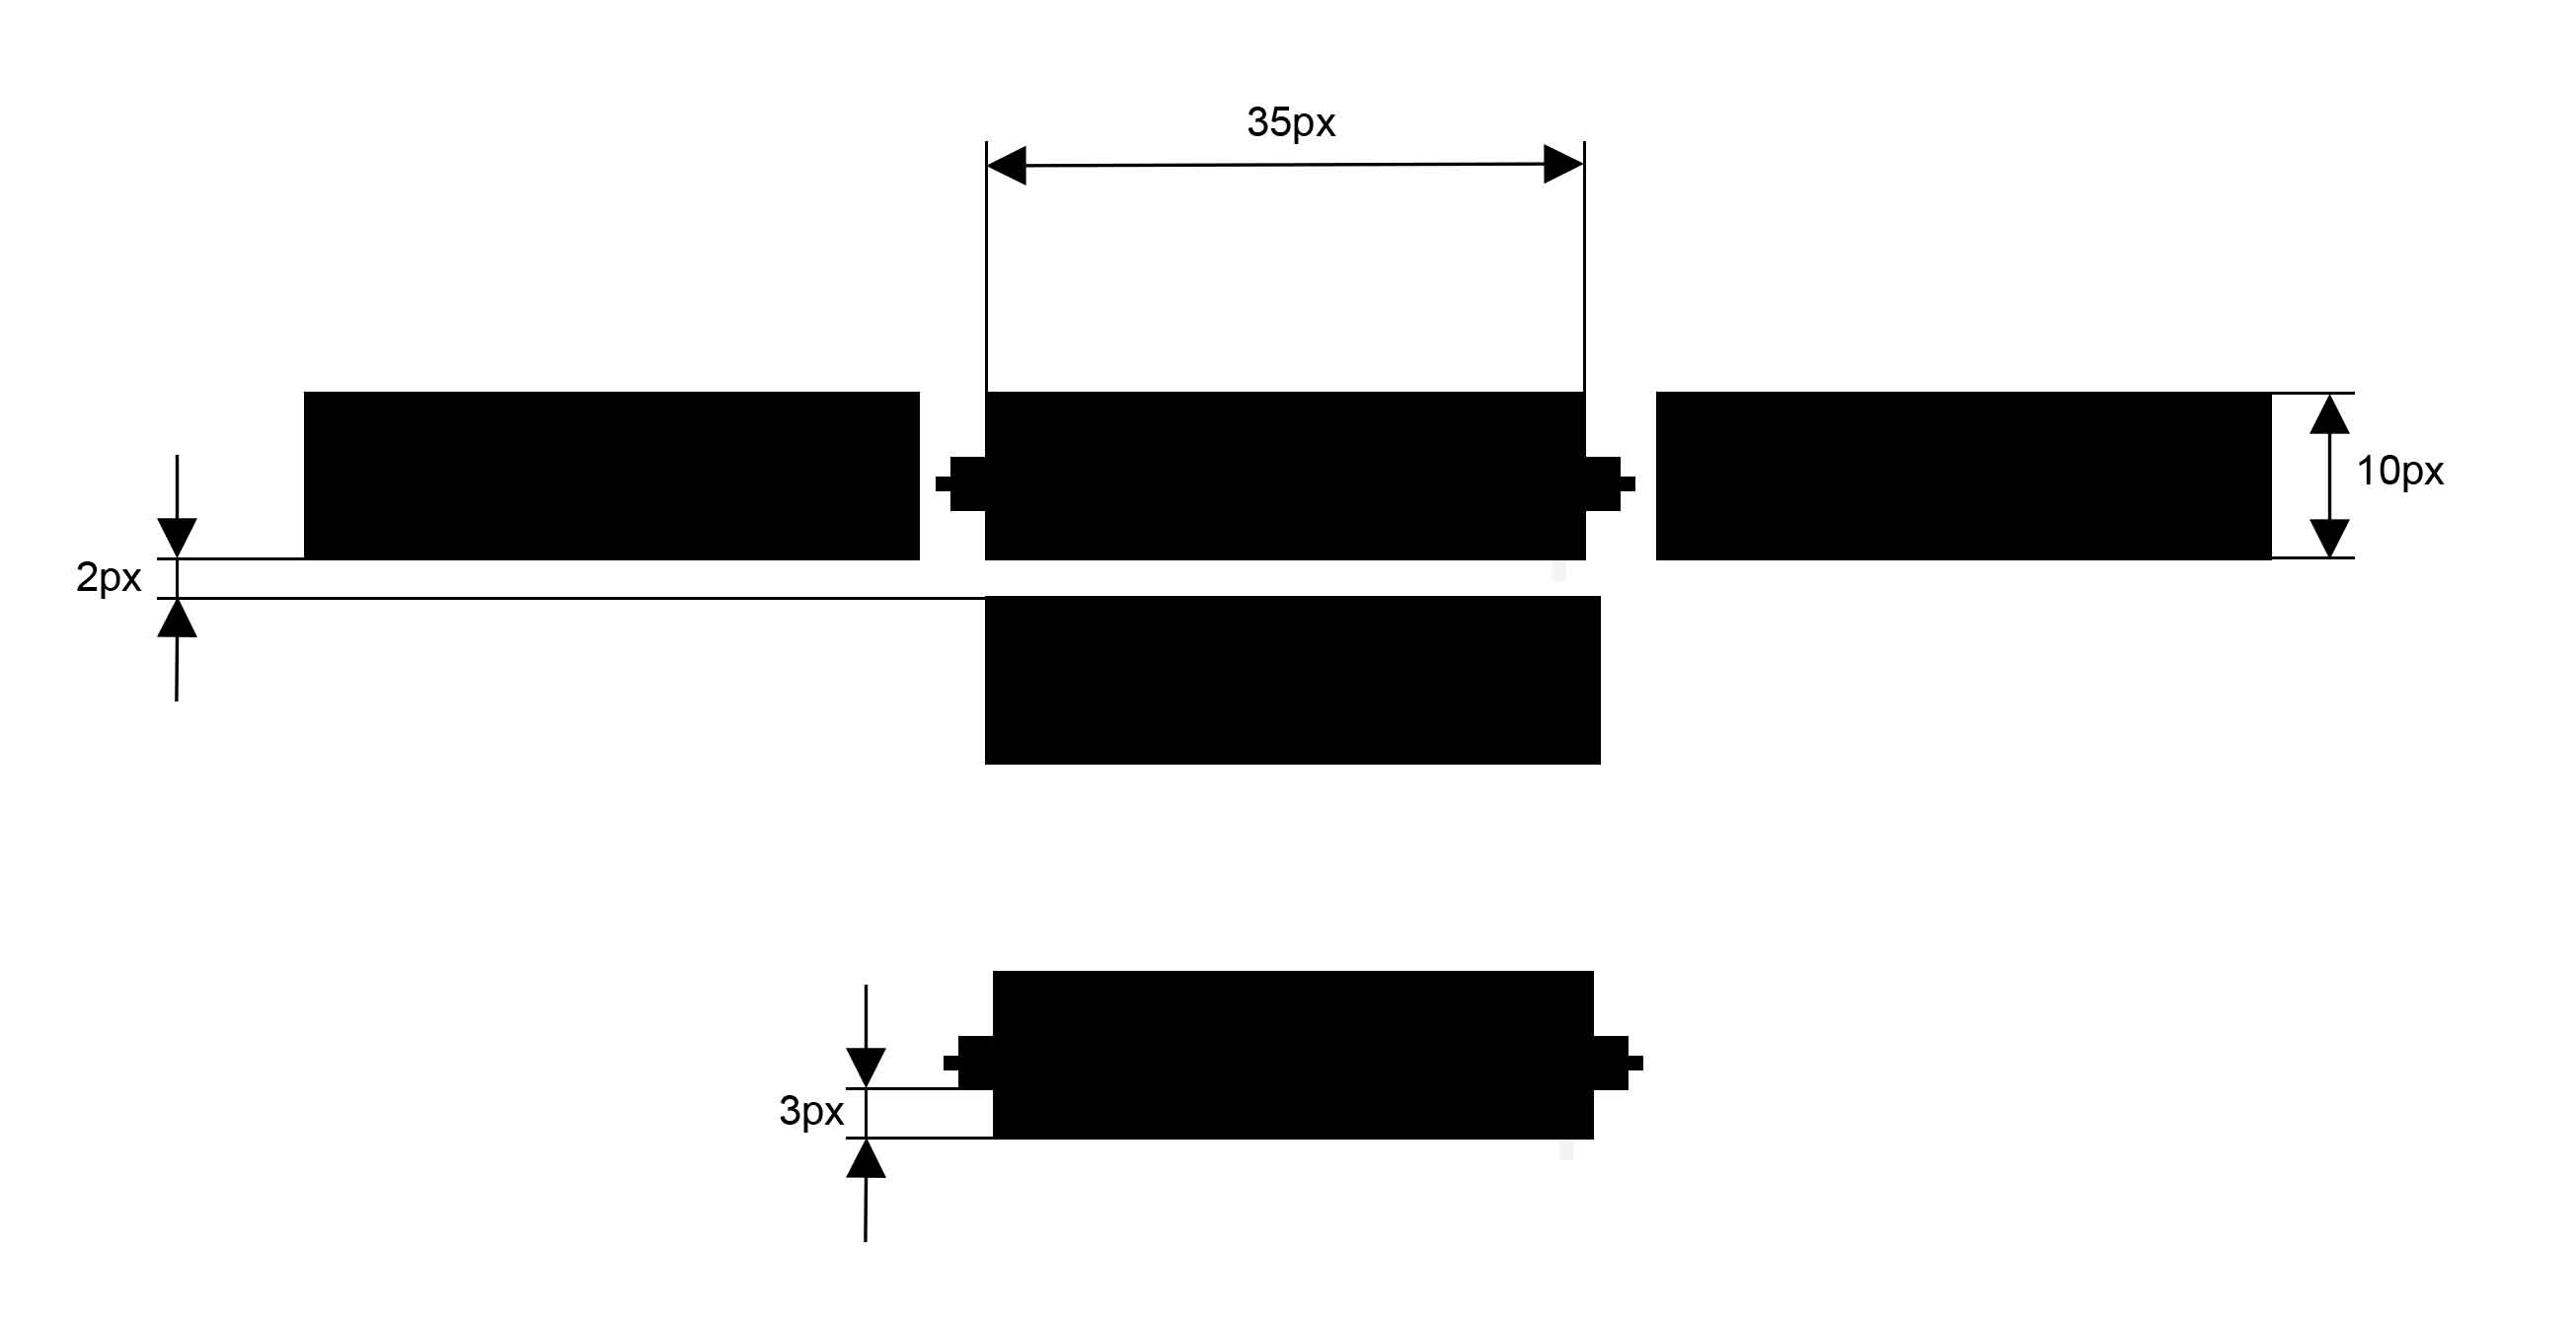
\includegraphics[width=1\linewidth]{measurement-and.jpg}
    \caption{First working AND gate}
    \label{fig:and-gate}
\end{figure}

The design of the detector (Fig. \ref{fig:and-gate}) implies that there is no max size for the length of the coincidence medium in the detector circuit as the waves have a width equal to the width of the coincidence channel.
\begin{tcolorbox}[colback=red!5!white,colframe=red!75!black,title=Assumption]
    The size of the Petri dish is \textbf{assumed} to be unsubstantially larger than the size of the chemical circuit inside of it. Continuing from both sizes are referred to interchangeably.
\end{tcolorbox}
A significant milestone in the practical application of chemical computing was achieved through the real-life implementation of an AND gate using the Belousov-Zhabotinsky (BZ) reaction. This implementation, detailed by \cite{gorecki2003chemical} and shown in Figure \ref{fig:bz-and-gate}, serves as a cornerstone example of how chemical reactions can be harnessed for computational purposes.

\begin{figure}
    \centering
    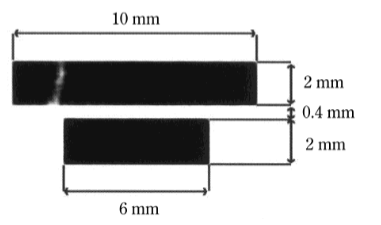
\includegraphics[width=0.6\linewidth]{images/Screenshot 2024-03-10 at 20.59.51.png}
    \caption{Real-life AND gate using BZ reaction \citep{gorecki2003chemical}}
    \label{fig:bz-and-gate}
\end{figure}


Now, this is just a simulation we are doing, so to get the mapping for a real Petri dish, we can use the dimentions of the gate in a Petri dish. 
In \cite{gorecki2003chemical}, the exact dimensions in mm of the collision detector, signal channel of 10cm, and a membrane filter of 2.5cm inside of the Petri dish are specified. These dimensions can be used to map it to the one in our simulation.


Given the following mapping from real life measurements to simulation pixels:
\begin{itemize}
    \item Stripe width: \(2 \text{ mm} = 10 \text{ px}\)
    \item Channel gap: \(0.4 \text{ mm} = 2 \text{ px}\)
\end{itemize}

We can establish a scaling factor for the conversion from millimeters to pixels.
For the stripe width:
\[ \text{Scaling factor} = \frac{10 \text{ px}}{2 \text{ mm}} = 5 \text{ px/mm} \]

For the channel gap:
\[ \text{Scaling factor} = \frac{2 \text{ px}}{0.4 \text{ mm}} = \frac{2 \text{ px}}{\frac{2}{5} \text{ mm}} = 5 \text{ px/mm} \]

Thus, both measurements confirm the same scaling factor. Using this consistent scaling factor, we can convert any measurement from millimeters to pixels.

Using this scaling factor, we can convert any measurement from millimeters to pixels.
For a dimension of \(10 \text{ mm} \times 4.4 \text{ mm}\), the conversion would be:

\begin{align*}
\text{Width in pixels} &= 10 \text{ mm} \times 5 \text{ px/mm} = 50 \text{ px} \\
\text{Height in pixels} &= 4.4 \text{ mm} \times 5 \text{ px/mm} = 22 \text{ px}
\end{align*}

Thus, a real-life size of \(10 \text{ mm} \times 4.4 \text{ mm}\) would map to a size of \(50 \text{ px} \times 22 \text{ px}\) in the simulation.
More importantly, the simulation uses details as small as $1\text{px}^2$, which would amount to $\frac{1}{5}\text{mm}^2$ in real life, which would be infeasible because details smaller than $1\text{mm}^2$ are difficult to control accurately.
This means we would need to scale the simulation up in order to have details easier to control. 
However, as we scale it up, the surface area of the Petri dish becomes larger and the angle of incidence of the light becomes more significant, which is a problem we will explore later on in section \ref{sec:light-imperfections}.
The reason there is a section before that is because \todo{help}


\section{Finding $\phi_{\text{min}}$ and $\phi_{\text{max}}$ for a Chemical Diode} \label{sec:finding-phi-min-max}
As mentioned in equation \ref{eq:u-partial-t}, $\phi$ is external illumination that creates the chemical circuit. It sets the value of $\phi$ to either $\phi_{\text{active}}$ or $\phi_{\text{passive}}$. 
$\phi$ values control the lighting conditions of the chemical circuit.
Active regions are where it is dark/unilluminated and passive regions are where there is light/illlumination.
The reason behind the need to measure the $\phi$ values for a Chemical Diode stems from the fact that a chemical diode is less sensitive to changes in $\phi$ values than other chemical components.
This means that the diode can still operate even outside the values for $\phi$ established in literature. In order to see where chemical computers break, we need to measure each component and see where it breaks.
The operational range for a whole computer is the intersection of the operational ranges of every component, which is equal to that of the most sensitive performing component.
Here $\phi_{\text{passive}}$ is measured at different values because that is the value controlling the illuminated area, which makes the circuit there ``passive''. This simulates less illumination of light at the diode, altering its behaviour.
\subsection{Measuring $\phi_{\text{min}}$, $\phi_{\text{max}}$}


During the evaluation of $\phi_{\text{min}}$, $\phi_{\text{max}}$, the diode had to be tested from numerous directions to determine the minimum and maximum values of $\phi_{\text{passive}}$ where it still functions correctly as a diode, 
which means that it passes waves from right to left, but never from left to right. As we approach the limits, new cases start appearing where the wave becomes able to pass through from a very specific angle that changes as we change the phi value, 
making it impossible to automatically test, so manual testing was needed to verify if the diode works in every single use case for the limit phi values. Also, the minimum and maximum values start to highly depend on the testing conditions, 
and whether the diode works or not starts to depend on how you are using it; for example, do you start a wave right at the diode? 
If not, what is the minimum distance the diode has to work for? This greatly changes the minimum and maximum phi values. 
\subsubsection*{Measurement Methodology}
The measurement was done by starting a wave at a distance from the diode and measuring if it passes through the diode. 
it's done from both directions.
tested from multiple angles and distances and qualitatively assessed if it still performs as a diode under every single case.
The investigation is trying to establish $\phi_{\text{min}}$ and $\phi_{\text{max}}$ for the diode, which are the operational boundaries for the $\phi_{\text{passive}}$ values that the diode can tolerate, 
which represent the less than ideal lighting conditions are are trying to explore.
we know that the diode operates mostly at $\phi_{\text{passive} = \phi_{\text{literature}}} = 0.0975$. 
We start from this value and start going in both directions, increasing and decreasing the value of $\phi_{\text{passive}}$ and measuring if the diode still works.
$\phi_{\text{current}} = \phi_{\text{literature}} = 0.0975$
\begin{algorithm}
    \caption{Detailed $\phi$ Exploration Algorithm. It works by starting from $\phi_{\text{literature}}$ and searching for the last value where the diode still works. 
    The function \text{TestDiode} returns true if the diode works and false if it does not. This is done manually by performing comprehensive tests on the diode from both directions. 
    It should let the wave through from right to left, but never from left to right. This shall be true for all angles and distances.
    The whole algorithm is run manually and is written out here just for illustrative purposes.}
    \label{alg:phi-exploration}
    \begin{algorithmic}[1]
        \State $\phi_{\text{current}} \leftarrow \phi_{\text{literature}}$
        \State $precision \leftarrow 0.5$ \Comment{Starting precision}
        \State $step \leftarrow 0.05$ \Comment{Initial step size}
        \While{$precision \geq 0.0001$} \Comment{Continue until precision is fine enough}
            \State $found \leftarrow$ \textbf{false}
            \While{\textbf{not} $found$}
                \If{\text{TestDiode}($\phi_{\text{current}} + step$)}
                    \State $\phi_{\text{current}} \leftarrow \phi_{\text{current}} + step$
                \ElsIf{\text{TestDiode}($\phi_{\text{current}} - step$)}
                    \State $\phi_{\text{current}} \leftarrow \phi_{\text{current}} - step$
                \Else
                    \State $found \leftarrow$ \textbf{true}
                \EndIf
            \EndWhile
            \State $precision \leftarrow precision / 10$ \Comment{Increase precision}
            \State $step \leftarrow 0.5 * precision$ \Comment{Adjust step size based on new precision}
        \EndWhile
        \State $\phi_{\text{functional}} \leftarrow \phi_{\text{current}}$
    \end{algorithmic}
\end{algorithm}


Algorithm \ref{alg:phi-exploration} outlines the process of finding the boundaries of $\phi_{\text{passive}}$ for the diode. It is run twice, 
once with \verb|step=0.05| and once with \verb|step=-0.05| to go in the other direction.

\subsubsection*{Results}

Results of measurement: 
\begin{itemize}
    \item $\phi_{\text{max}} = 0.106127$
    \item $\phi_{\text{min}} = 0.09555$
\end{itemize}

That is, as long as $\phi_{\text{min}} < \phi_{\text{passive}} < \phi_{\text{max}}$, then the diode will function as expected, even though the propagation time would still be affected (as seen in Figure \ref{fig:phi_passive_propagation_times}), causing synchronisation problems in larger circuits.


\subsection{Propagation Time Variation of the Diode Under Different Lighting Conditions}\label{sec:propagation-time-variation}
The reason we are looking at propagation time varyiation is because if that changes in response to the lighting conditions,
then the diode will behave as expected, but larger circuits that synchronise with the output of that diode and other chemical components
will be affected by this change and might not work as expected.
\subsubsection*{Methodology}
The way the experiment was set up was that a diode was set up in Figure \ref{fig:diode_experiment} where a wave was launched 25 px from the diode to allow it to pass through the diode and reach a small white flag where the wave is expected and the experiments are evaluated. A step in the diagram means one simulation pass. The parameters of the experiment were the following:
\begin{itemize}
    \item Number of $\phi_{\text{passive}}$ values: 30, of which only 19 succeeded, the remaining 11 could not pass through the diode due to the parameter being too out of range.
    \item Interval size: 0.0013448276
    \item Number of runs per $\phi_{\text{passive}}$ values: 7
    \item $\phi_{\text{start}}$: 0.08066608
    \item $\phi_{\text{end}}$: 0.121010914, never reached because once a wave passes through the diode, the concentration no longer reaches zero fully and that leaves a very small amount of inhibitor at the diode and due to the borderline value of $\phi_{\text{passive}}$ the next waves never manage to penetrate to get measured, so the highest measured value for $\phi_{\text{passive}}$ is 0.10487298
    \item Wave start: 39px before diode, which was observed to be enough to allow for the proper formation of the wave
    such that it can pass through the diode.
    \item Wave measure: 31px after diode, which was far away enough to measure a fully formed wave, provided
    that one passed through the diode. 
    \item $dt$: 0.001, also serves as a reference point for the amount of steps.
    \item Measurement interval: about every 5 steps, depending on the GPU frame rendering schedule
\end{itemize}

It is possible to run the experiment much more accurately, eliminating the need for multiple runs for the same $\phi_{\text{passive}}$ value we measured at every step and did not simulate another step in the simulation until the measurement was complete. However, that would drastically slow down the experiment, making it run for hours instead of minutes. For the purposes of merely showing that the propagation changes along with the slope, it was enough accuracy, so the faster and more inaccurate solution was chosen.

\begin{figure}
    \centering
    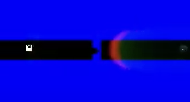
\includegraphics[width=0.5\linewidth]{diode.png}
    \caption{Diode Experiment}
    \label{fig:diode_experiment}
\end{figure}

So, the following limitation were found while working with the simulation. Due to the act that in metal sampling is a rendering operation, it cannot be done during the computation of the simulation. That means that I would have to synchronise it to run with rendering speed, but that would make the simulation too slow to run many experiments. It uses the step speed of the simulation, 1 frame = about 150 steps in the simulation. This is still accurate enough. I ran at $dt=0.001$.
To get better results the computation was run at $dt=0.001$ was done every 300 microseconds.
Additional values were added in between $\phi_{\text{min}}$ and $\phi_{\text{max}}$ where the curve started to change, and the results can be seen in Figure \ref{fig:phi_passive_propagation_times_detail_max}.

\subsection{Results}

The results of the experiment can be seen in Figure \ref{fig:phi_passive_propagation_times}. The propagation time decreases as there is less light, indicated by the decrease in the value of $\phi_{\text{passive}}$ and the reverse. This is to be expected, as a lower value brings it closer to $\phi_{\text{active}}$ (darkness), and illumination is an inhibitor. 
The reason the circuit has a higher tolerance to less light, compared to more light, is because the diode is much more resistant in the reverse direction as the wave has to go through a reverse triangle, 
which is specifically made to stop the propagation of waves. 
The diode also has a high tolerance to $\phi_{\text{passive}}$ increasing due to an additional spike added to the diode, which helps weaves to cross the gap easier, even when there is more light. The reason for $\phi_{\text{max}} < \phi_{\text{end}}$, meaning the diode was still letting the wave through left to right and not right to left at $\phi_{end}$, but it was not at other angles when tested, so the experiment measured propagation time, but the diode was only partially functional at these values

\begin{figure}
    \centering
    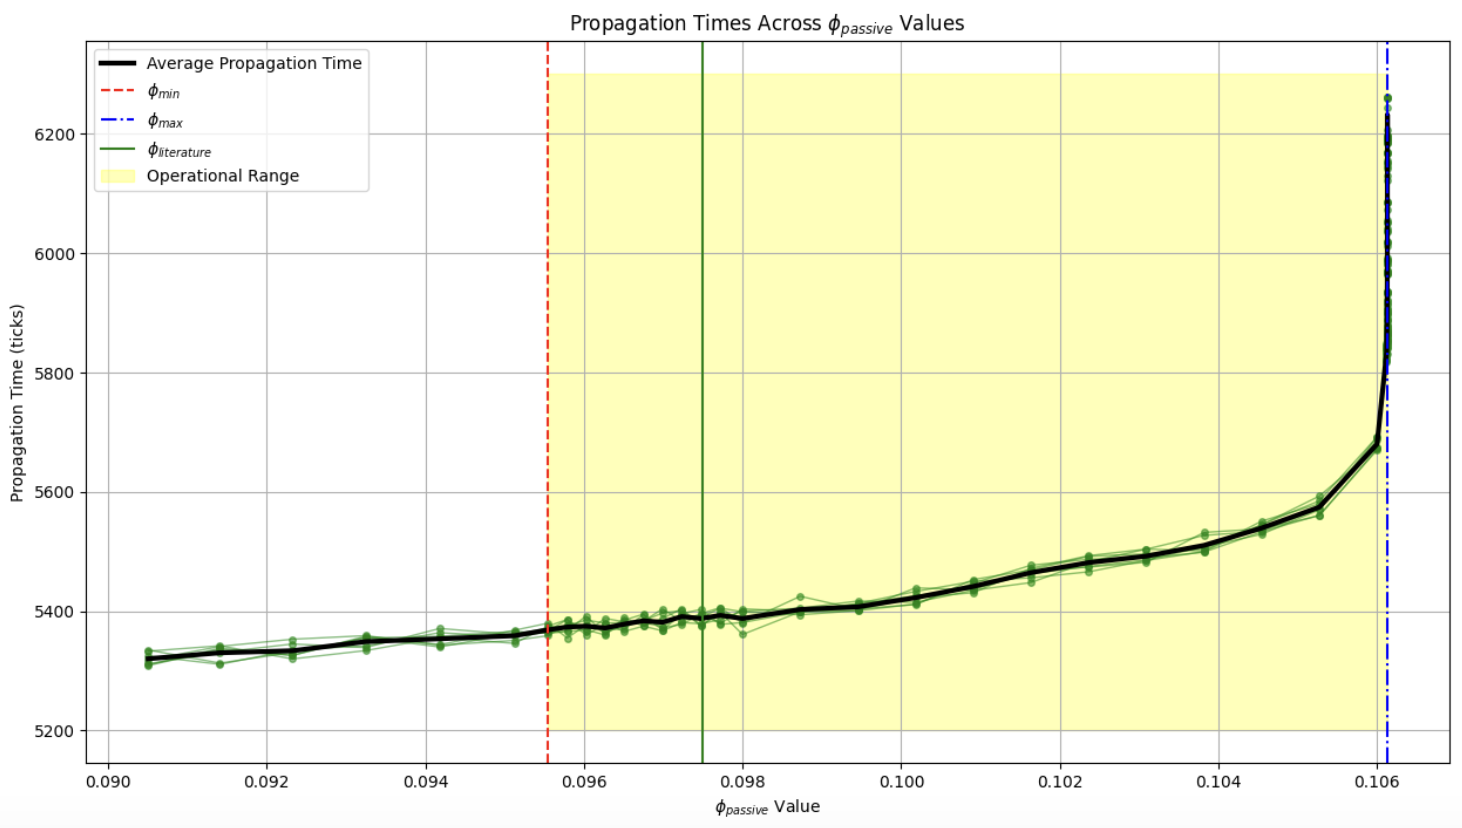
\includegraphics[width=\linewidth]{Screenshot 2024-03-09 at 10.35.01.png}
    \caption{Propagation times for various $\phi_{\text{passive}}$ values within the limits of $\phi_{\text{min}}$ and $\phi_{\text{max}}$, 
    illustrating the experimental outcomes of testing a diode in a Belousov-Zhabotinsky reaction. 
    Each point represents a propagation time measurement for a given $\phi_{\text{passive}}$, 
    with the average propagation time across measurements shown by a thicker black line. 
    The shaded area between $\phi_{\text{min}}$ (red dashed line) and $\phi_{\text{max}}$ (blue dashed line) highlights the range 
    where the diode works correctly, with the $\phi$ used commonly in literature marked by a solid green line.}
    \label{fig:phi_passive_propagation_times}
    
\end{figure}

\begin{figure}
    \centering
    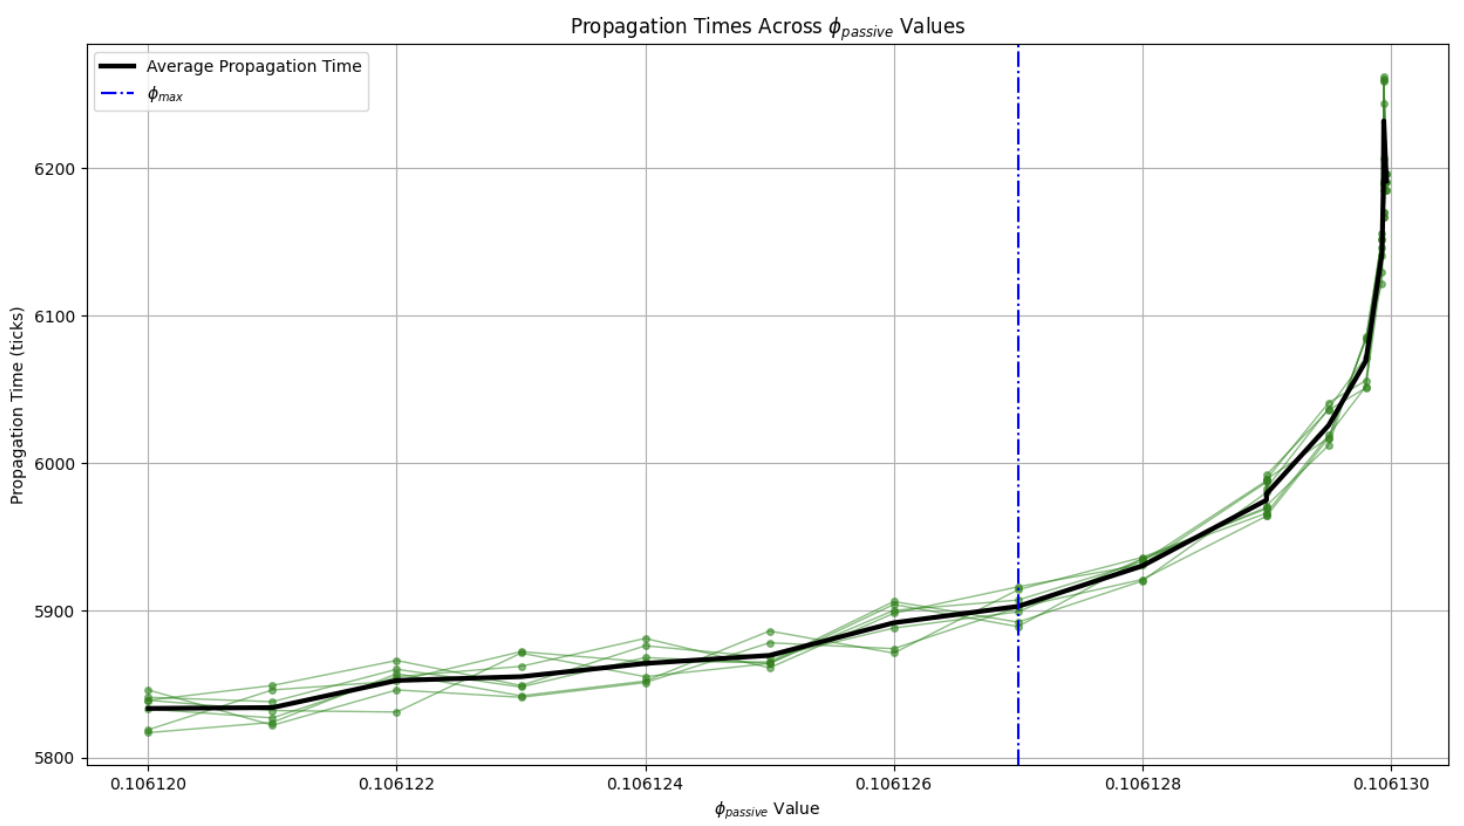
\includegraphics[width=1\linewidth]{Screenshot 2024-03-10 at 07.50.59.png}
    \caption{Propagation times around the value of $\phi_{\text{max}}$. The range of $\phi$ is $\phi_{\text{max}} - 7 \times 10^{-6} \leq \phi \leq \phi_{\text{max}} + 3 \times 10^{-6}$}
    \label{fig:phi_passive_propagation_times_detail_max}
\end{figure}



\begin{figure}
	\centering
	\begin{subfigure}{0.24\textwidth}
		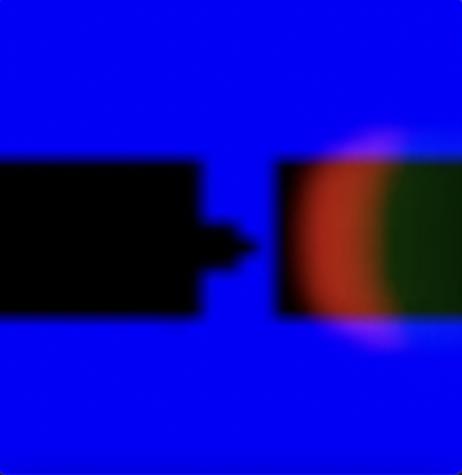
\includegraphics[width=\linewidth]{diode/easy/Screenshot 2024-03-09 at 16.21.56.png}
		\caption*{$t = 1$}
	\end{subfigure}
	\begin{subfigure}{0.24\textwidth}
		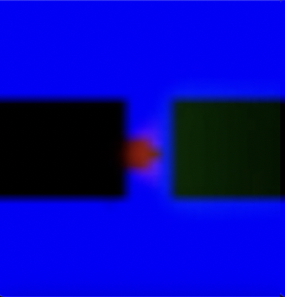
\includegraphics[width=\linewidth]{diode/easy/Screenshot 2024-03-09 at 16.22.24.png}
		\caption*{$t = 2$}
	\end{subfigure}
    \begin{subfigure}{0.24\textwidth}
		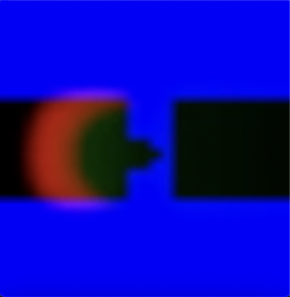
\includegraphics[width=\linewidth]{diode/easy/Screenshot 2024-03-09 at 16.22.35.png}
		\caption*{$t = 3$}
	\end{subfigure}
    \begin{subfigure}{0.24\textwidth}
		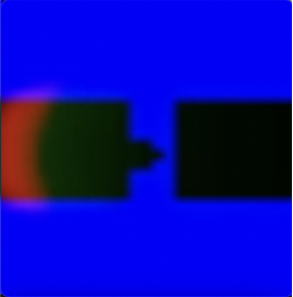
\includegraphics[width=\linewidth]{diode/easy/Screenshot 2024-03-09 at 16.22.45.png}
		\caption*{$t = 4$}
	\end{subfigure}

	\begin{subfigure}{0.24\textwidth}
		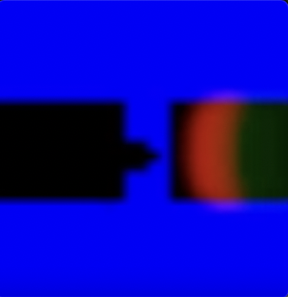
\includegraphics[width=\linewidth]{diode/hard/Screenshot 2024-03-09 at 16.23.41.png}
		\caption*{$t = 1$}
	\end{subfigure}
	\begin{subfigure}{0.24\textwidth}
		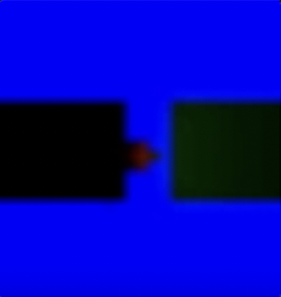
\includegraphics[width=\linewidth]{diode/hard/Screenshot 2024-03-09 at 16.23.48.png}
		\caption*{$t = 2$}
	\end{subfigure}
    \begin{subfigure}{0.24\textwidth}
		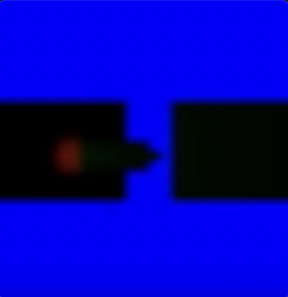
\includegraphics[width=\linewidth]{diode/hard/Screenshot 2024-03-09 at 16.23.55.png}
		\caption*{$t = 3$}
	\end{subfigure}
    \begin{subfigure}{0.24\textwidth}
		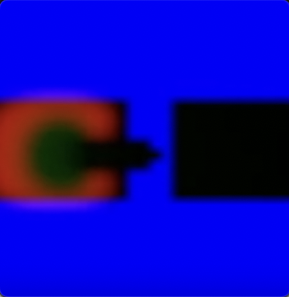
\includegraphics[width=\linewidth]{diode/hard/Screenshot 2024-03-09 at 16.24.01.png}
		\caption*{$t = 4$}
	\end{subfigure}

	\caption{Comparison of two waves passing through a diode. Above $\phi_{\text{passive}} = \phi_{\text{literature}}$, below $\phi_{\text{passive}} = \phi_{max}$. Both have different propagation speeds, so they have been equalised for the purpose of comparing their interaction with the diode side by side. The second wave takes substantially more time to form and is about 700 time steps slower as seen in Figure \ref{fig:phi_passive_propagation_times_detail_max}, which is quite a lot in such simulations.}
	\label{fig:comparison_diode}
\end{figure}

% \section{Calculating Possible Movement of the Light Source}
\section{Estimating The Light Source's Position}\label{sec:light-imperfections}



Identifying the minimal operational conditions for the AND gate in real life involves examining light intensity, angle of incidence, and the effect of the thickness of the beam of light on the BZ reaction.


Some circuits \todo{is it the same reaction} can be influenced by temperature, such as \cite{yamada2022artificial}, which uses a more complex model of the oregonator.  .


Shining light on the BZ surface: \citep{barry1979methods}
The catalyst in these reactions is light, using light we can modulate the speed using $\Phi$.
A light bulb is shined over the Petri dish (fig. \ref{fig:light-over-petri})

Given multiple light sources, the total illumination $I_{\text{total}}$ at a point on a surface is the sum of the illuminations from each individual light source (fig. \ref{fig:light-flux-petri-dish}). The illumination $I_i$ from a single source at a given point is given by the inverse square law, adjusted for the angle of incidence $\theta_i$:

\[
I_{\text{total}} = \sum_{i=1}^{n} \frac{P_i}{4\pi r_i^2} \cdot \cos(\theta_i)
\]

where $P_i$ is the power of the $i$-th light source, $r_i$ is the distance from the $i$-th light source to the point, and $\theta_i$ is the angle between the direction of the $i$-th light ray and the normal to the surface. The cosine term $\cos(\theta_i)$ accounts for the angle of incidence, with the intensity contribution from the light source decreasing as the angle increases.




\begin{figure}
    \centering
    \begin{subfigure}{.5\textwidth}
        \centering
        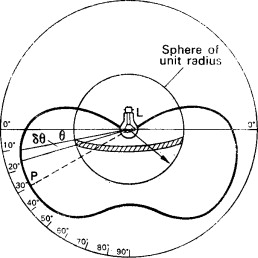
\includegraphics[width=\linewidth]{sphere2.jpg}
        \caption{Light shined over a petri dish}
        \label{fig:light-over-petri}
    \end{subfigure}%
    \begin{subfigure}{.5\textwidth}
        \centering
        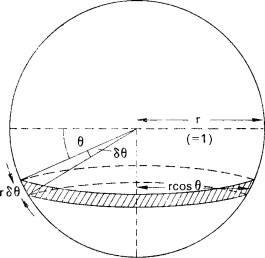
\includegraphics[width=\linewidth]{sphere.jpg}
        \caption{Light flux at different parts of a Petri dish}
        \label{fig:light-flux-petri-dish}
    \end{subfigure}
    \caption{Visualization of light interaction with a Petri dish \citep{edwards_1970}.}
\end{figure}
This means that now we can use that in the simulation to simulate the imperfections of light sources. 

Most uses a single light bulb to illuminate the Petri dish as the Petri dish is small. 

It is very important to calculate how far away the light source is from the Petri dish in order to make useful light calculations later on. This is because if the light source is very far away, the angle of incidence $\theta$ is very close to $90^\circ$, so the effect of the angle is insignificant.

In real experiments, the chemical reaction that occurs on the gel surface is sensitive to light due to the specific catalyst used (Ru(bpy)$_3$SO$_4$). 
However, to observe and record the process, they need to use light to illuminate the gel, so that the camera can capture images. The experiment design, including time-varying intervals of different light intensities, allows them to balance between controlling the reaction and capturing the activity on the gel. \cite{TOTH20091605}

They all project a single light bulb and then use a mask to have the shape they want projected, such that light does not kill off the reaction and there is light everywhere else. This is important to show how imperfections can affect the simulation . \cite{gorecki2003chemical}
An experimental setup for observing pulses in a photosensitive BZ reaction, as detailed in the work by Gorecki et al., is illustrated in the following Figure~\ref{fig:gorecki-setup}. This setup is crucial for understanding the dynamics of light-sensitive chemical reactions and their applications in computational models.

\begin{figure}[H]
    \centering
    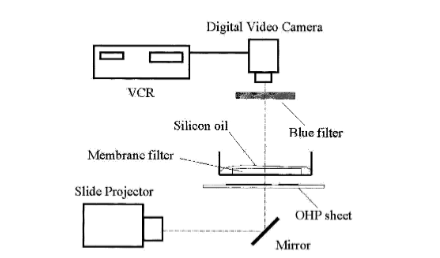
\includegraphics[width=0.7\linewidth]{images/Screenshot 2024-03-10 at 20.23.20.png}
    \caption{Experimental setup for observing pulses in a photosensitive BZ reaction \citep{gorecki2003chemical}.}
    \label{fig:gorecki-setup}
\end{figure}

\cite[71]{cui2004synchronization} contains a similar setup and goes into more detail how they project the pattern onto the gel. 
The book goes into more detail helpful for understanding the real-life environment where the waves propagate. 
One interesting observation is that the observation angle seems to change where we see the wave, which might be relevant for measuring the size of the waves, however this is not explored in this project.

\begin{tcolorbox}[colback=red!5!white,colframe=red!75!black,title=Assumption]
Unfortunately, \cite{gorecki2003chemical} do not specify how far away the light bulb projector is, which is used to illuminate the Petri dish, but we can assume the projector is far away, such that the angle of light projection is very close to $90^\circ$, making the effect of the angle insignificant. 
\end{tcolorbox}
We can still simulate that in our simulation to see what effect it would have if it were close to the medium; for larger circuits, this effect would be visible. Given a normal setup, what would be the maximum size of the Petri dish in a simulation before the effects of the light angle start to impact the simulation.




The distance between the active channel and the signal bar is 0.4 mm, which corresponds to exactly 2px in the simulation. 

Both stripes are 2 mm wide, the signal channel is 10 mm long, and the detector part is 6 mm long. The gap between the signal and the detector channels is 0.4 mm. The light intensity was selected so that the non-illuminated parts of the membrane were excitable, whereas the excitations died in the illuminated areas. In the experiment, the light intensity was set at I ) 24 kLx as determined by a light metre (ASONE LM-332), and the temperature was 295 $\pm$ 1 K \citep{gorecki2003chemical}.


From the provided information in the paper and the datasheet for the JCD100V-300W halogen bulb, we have the following data:

\begin{itemize}
    \item Luminous flux ($\Phi$) as specified in the datasheet = 6600\, $\text{lm}$ \citep{fujilamp2024jdc}
    \item Light intensity (I) at the Petri dish = 24,000\, $\text{lux}$
\end{itemize}

Originally, we calculated the luminous flux using the estimated luminous efficacy of 17 $\frac{\text{lm}}{\text{W}}$ and the power of the bulb (P) as 300 W, which gave us:
\[
\Phi_{\text{estimated}} = \text{Power of bulb} \times \text{Luminous efficacy} = 300\, \text{W} \times 17\, \frac{\text{lm}}{\text{W}} = 5100\, \text{lm}
\]
However, this was an approximation. The datasheet for the bulb specifies a luminous flux of 6600 lm, which suggests that our assumption for the luminous efficacy was incorrect.

Using the inverse square law, which relates the light intensity (I) to the distance (r) from the light source, we have:
\[
I = \frac{\Phi}{4\pi r^2}
\]
Solving for the distance (r) with the correct luminous flux, we get:
\[
r = \sqrt{\frac{\Phi}{4\pi I}}
\]
Substituting the values from the datasheet and the light intensity measurement, we find:
\[
r = \sqrt{\frac{6600\, \text{lm}}{4\pi \times 24,000\, \text{lux}}}
\]
\[
r \approx 0.148\, \text{metres}
\]

Thus, the corrected distance from the light source to the Petri dish, using the accurate luminous flux from the datasheet, is approximately 0.148 metres or 14.8 centimetres. This distance is crucial, as it suggests that the light intensity measurement of 24 kLux is likely taken close to the Petri dish where the biological samples are studied, rather than at an arbitrary point close to the light source.

\begin{figure}
    \centering
    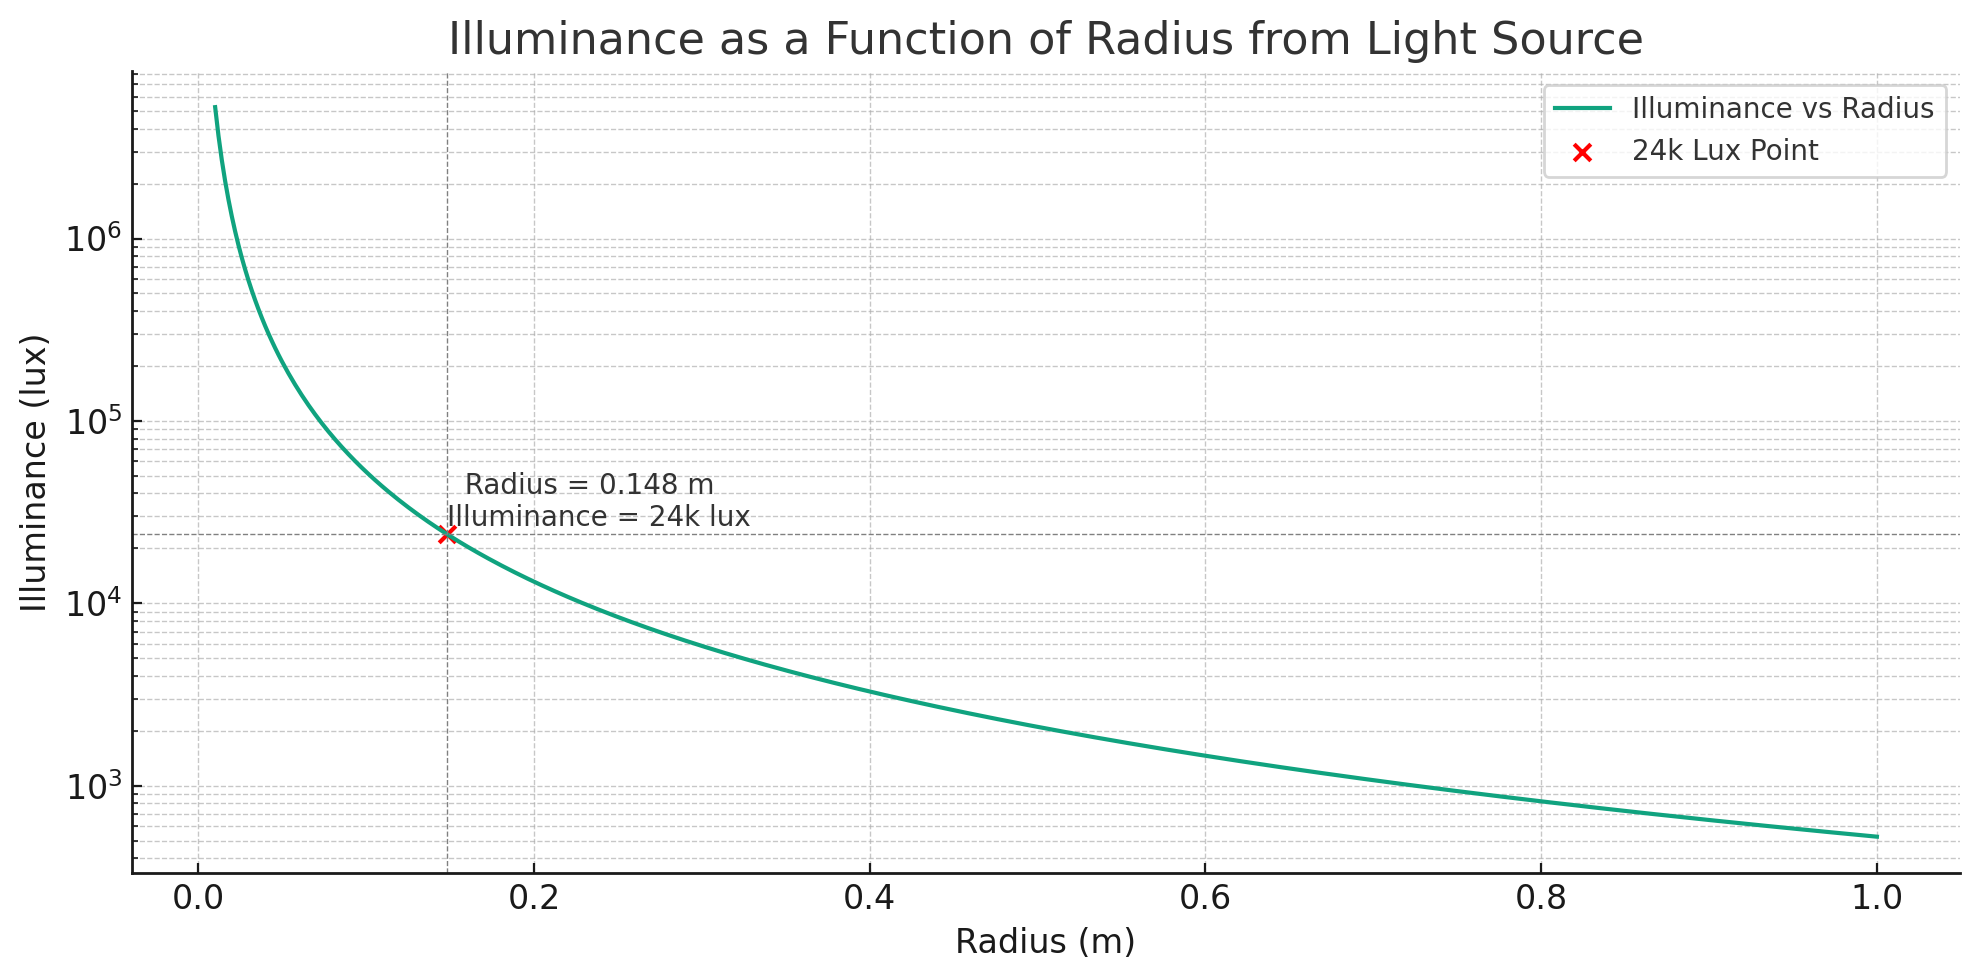
\includegraphics[width=\linewidth]{radius-illumination.jpg}
    \caption{Radius Illumination Graph}
    \label{fig:radius-illumination}
\end{figure}

In figure \ref{fig:radius-illumination} it is shown how the radius impacts the intensity at the light. 
Given the luminous flux \( \Phi \) of the JCD100V-300W bulb as 6600 lumens, we can calculate the illuminance \( I \) at various distances from the light source. The illuminance is given by the formula:
\[ I = \frac{\Phi}{4\pi d^2} \]
where \( d \) is the distance from the light source in meters.

For distances of 10 cm, 12 cm, 18 cm, and 20 cm, the illuminance values calculated are:

\begin{itemize}
    \item At 10 cm: \( I \approx 52521 \) lux
    \item At 12 cm: \( I \approx 36473 \) lux
    \item At 18 cm: \( I \approx 16210 \) lux
    \item At 20 cm: \( I \approx 13130 \) lux
\end{itemize}

These values illustrate a significant change in illumination as the radius increases, indicating that the radius is a crucial factor in determining the intensity of light received at a point.

Concluding from these calculations, it is likely that the measurement of 24 kLux was made relatively close to the Petri dish. This is because the light intensity of 24 kLux is a practical measure for the conditions under which biological samples are typically studied. Measuring illuminance right next to the light source would yield an impractically high value, which is not as useful for experimental purposes. Hence, the measurement taken is more likely to be representative of the actual working conditions near the Petri dish.


\section{Estimating The Maximum Petri Dish Size for a Chemical Diode \citep{gorecki2003chemical}} \label{sec:computer-size-limitations}


Next thing is to add the imperfection in the simulation with only an AND gate. To do that, I need to come up with a formula about plugging in a pixel and getting out the illumincation percentage. 
The percentage is basically the $\cos\theta$ as it is 0 when the angle is $90^\circ$.
let's assume a parallel light source is max intensity and an angle of 0 is no intensity at all, so in the formula we would plug in $\phi=0.054$ for when it's active and $\phi=0.0975$ when it's passive. Active means no light, passive means a lot of light, so when the light source becomes weak at a point, that would mean thath $\phi$ becomes more active. 
let's come up with a formula in mm that tells us when we move 1mm from the center of the petri dish where the light is most intense, what angle is that. That should be pretty simple, we have a right triangle, 
\begin{figure}
    \centering
    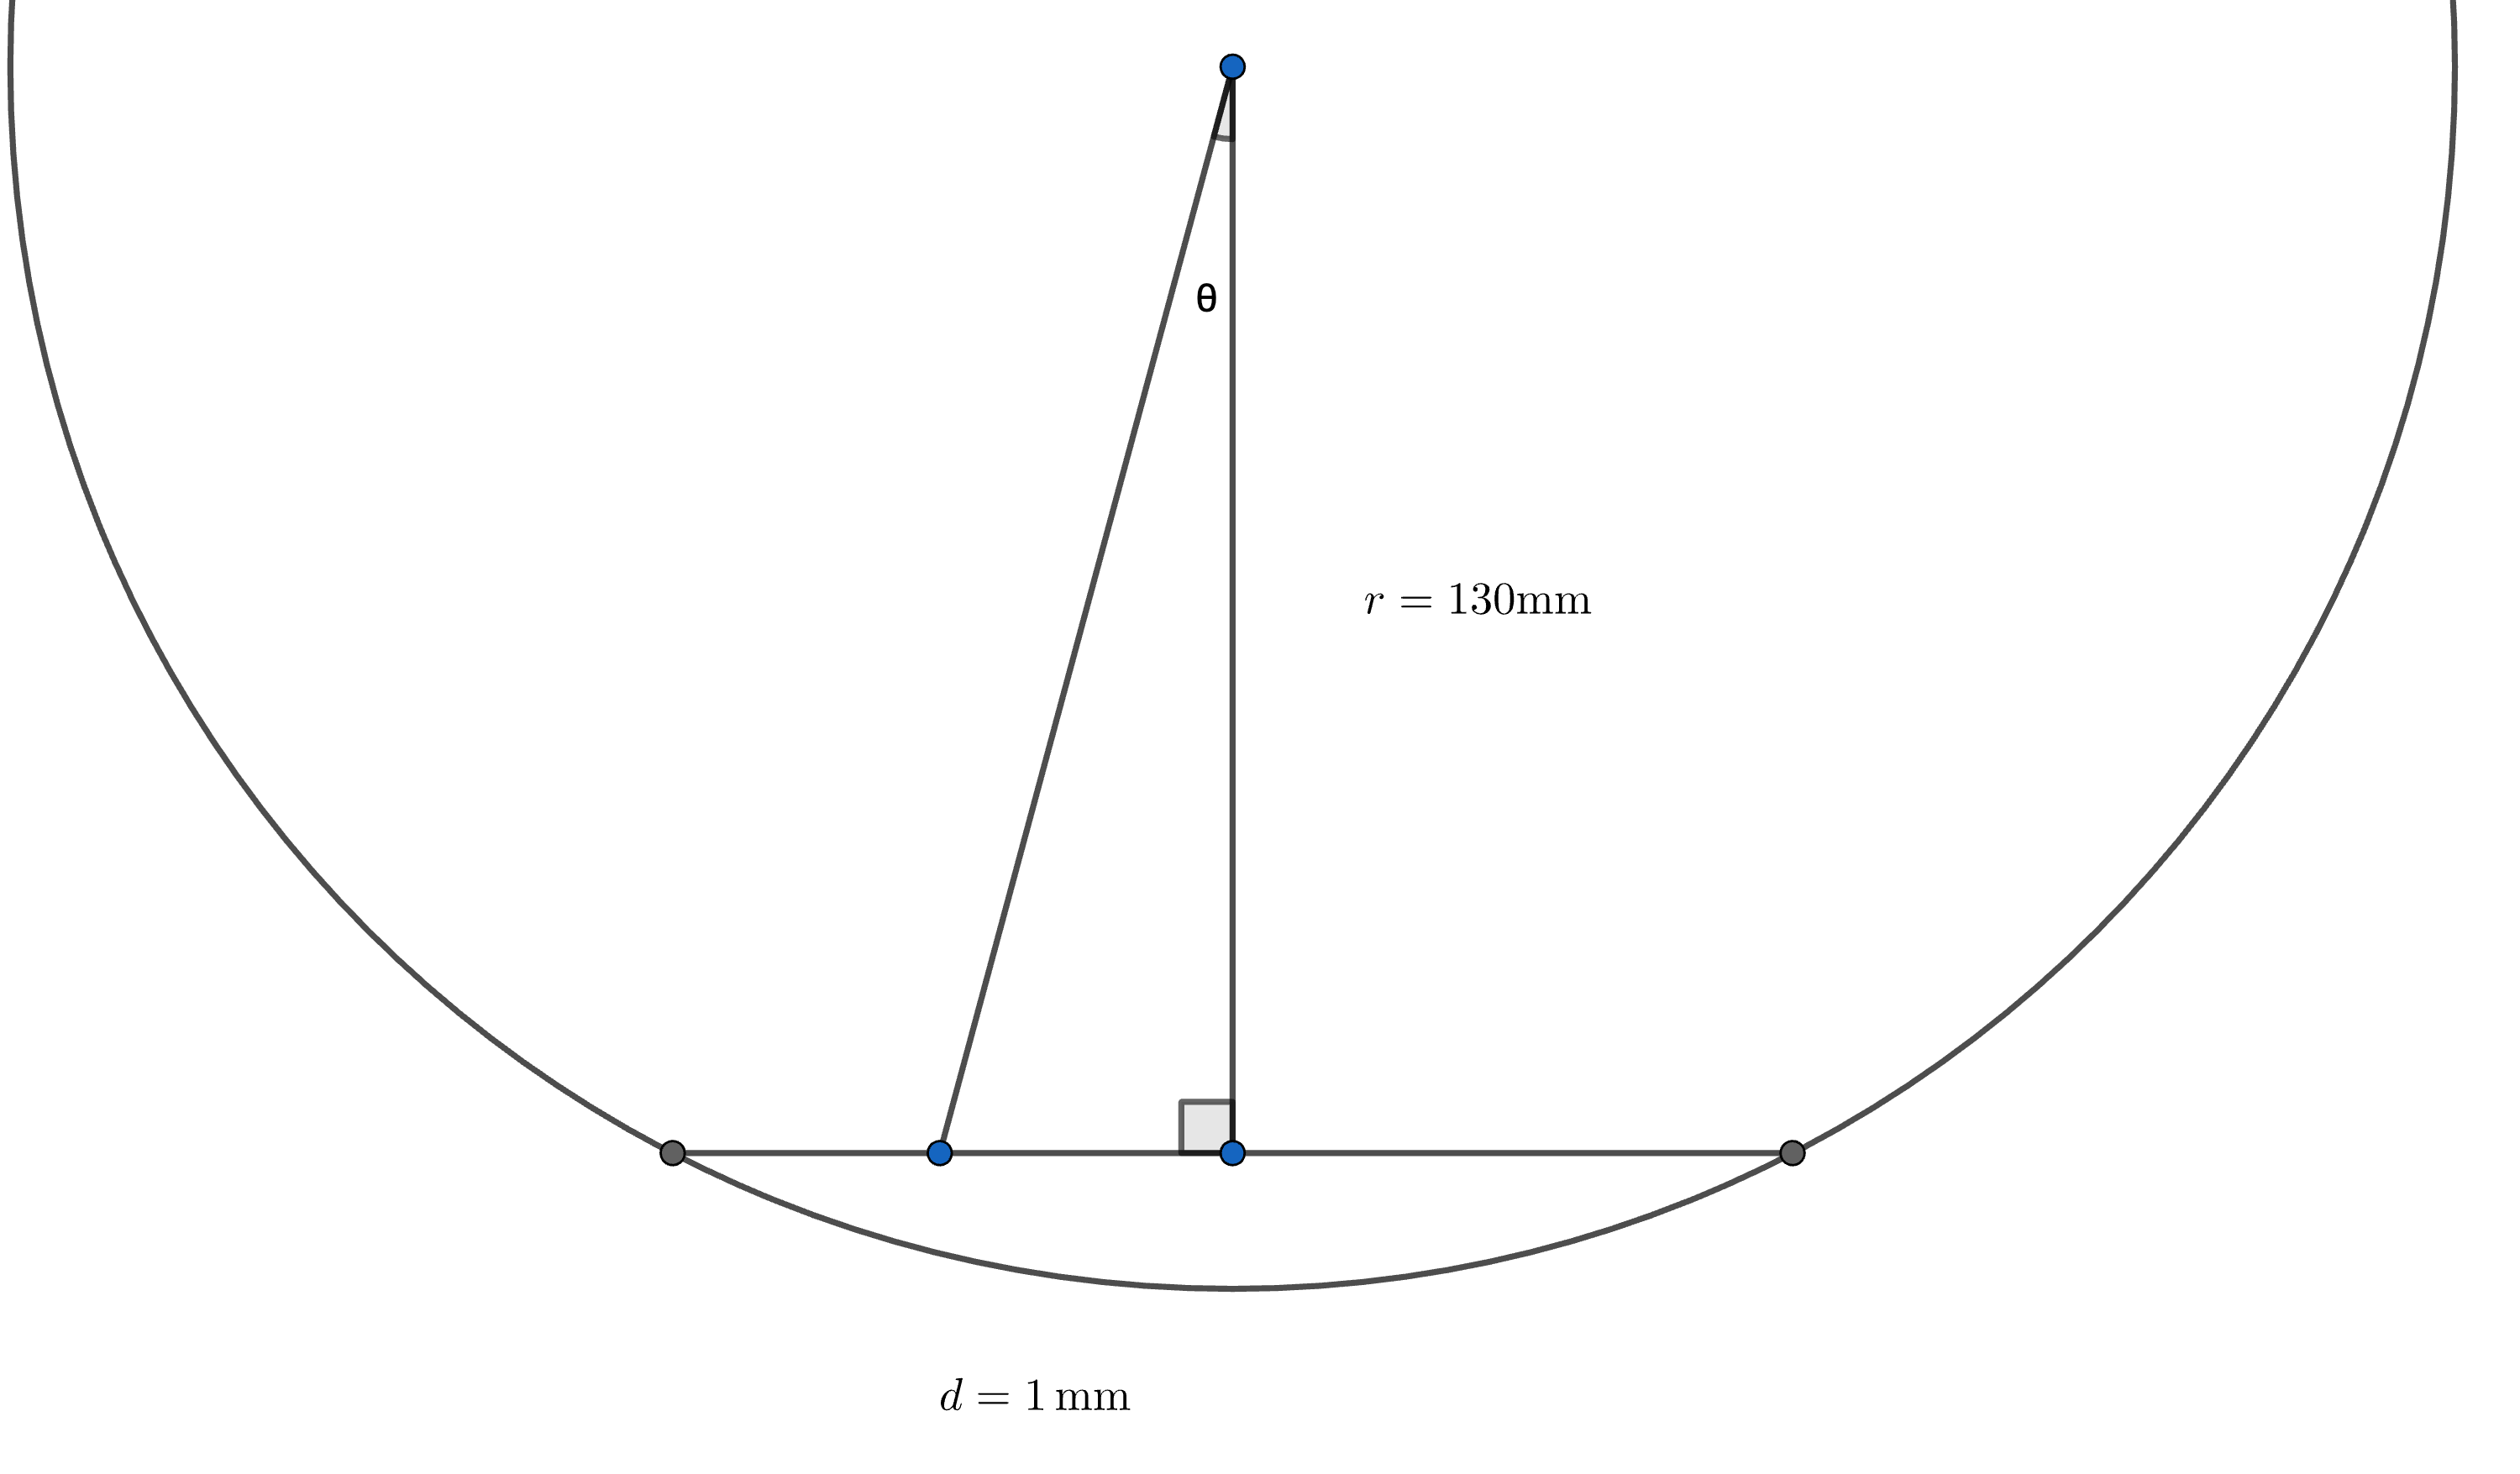
\includegraphics[width=1\linewidth]{geogebra-export (1).png}
    \caption{Illustration of finding the angle $\theta$}
    \label{fig:finding-theta}
\end{figure}

We have to find the angle every time when we move \( x \) mm from the center of the petri dish.

To calculate the angle \( \theta \) for any given radial distance \( r_c \) from the center of the Petri dish, we convert the pixel distance \( p \) to millimeters using the scaling factor \( s \) (in px/mm):

\[ r_c = p \times s \]

The angle \( \theta \) is then found using the arctangent function with respect to the height \( h \) of the light source above the center of the Petri dish:

\[ \theta = \arctan\left(\frac{r_c}{h}\right) \]

The percentage of illumination \( I_p \) at this radial distance is given by the cosine of \( \theta \):

\[ I_p = \cos(\theta) \]

Since \( \cos(\arctan(x)) \) simplifies, we can express \( I_p \) directly as:

\[ I_p = \frac{1}{\sqrt{1 + \left(\frac{r_c}{h}\right)^2}} \]

The real-world distribution of light as we get further away from the center of the Petri dish is illustrated in Figure~\ref{fig:illumination-percentage}.

\begin{figure}
    \centering
    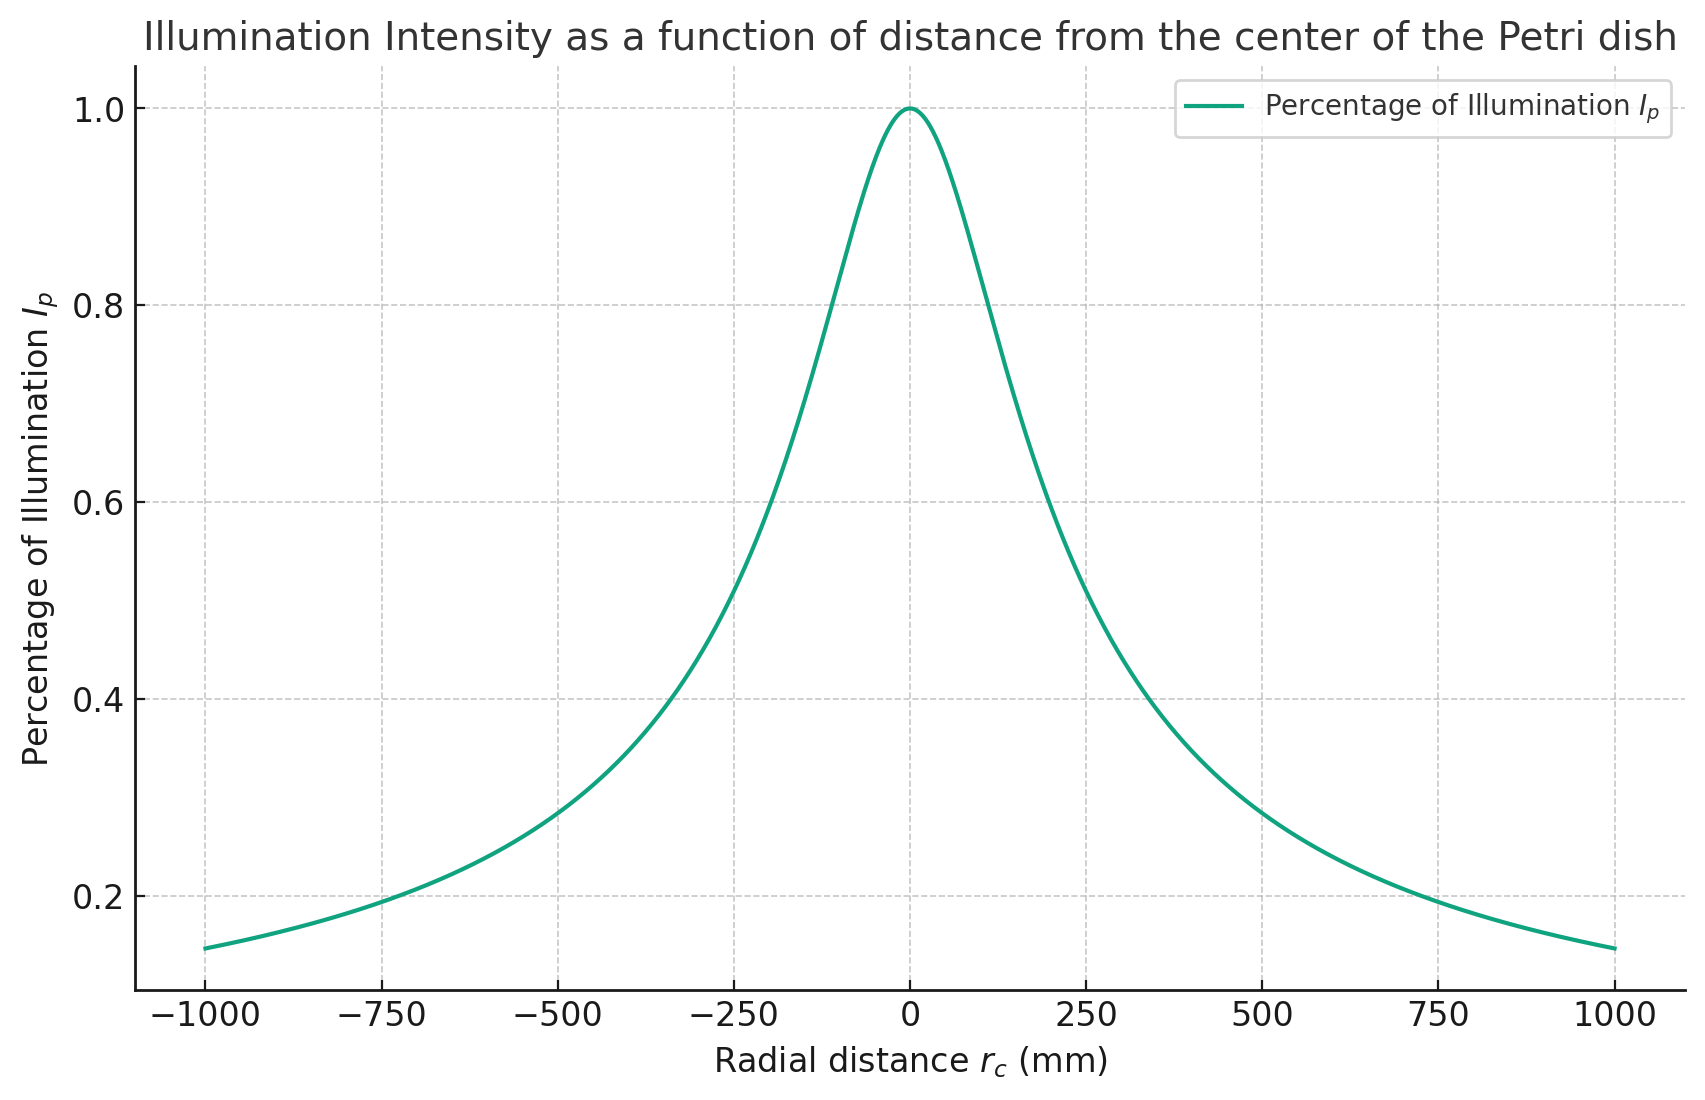
\includegraphics[width=1\linewidth]{images/831353b8-f4b4-4a93-9c41-ba3d6b6f5811.jpg}
    \caption{The graph represents the percentage of illumination $I_p$ as a function of the radial distance $r_c$ from the center of the Petri dish. The illumination percentage is calculated using the equation:$I_p = \frac{1}{\sqrt{1 + \left(\frac{r_c}{h}\right)^2}}$
    where \( r_c \) is the radial distance from the center of the Petri dish in millimeters, and \( h \) is the height of the light source above the center of the Petri dish, which is 148 mm. The graph extends from \( r_c = -1000 \) mm to \( r_c = 1000 \) mm to illustrate the symmetrical decrease in illumination intensity on both sides of the center point.}
    \label{fig:illumination-percentage}
\end{figure}



\begin{tcolorbox}[colback=red!5!white,colframe=blue!75!black,title=Assumptions for mapping light intensity to radial distance,label={ass:assumptions-light-intensity}]
    In our analysis, rather than directly calculating the rate of change of distance with respect to illumination intensity (\(\frac{dl}{d\phi}\)), we employ an interpolation strategy to estimate the illumination percentage between \(\phi_{\text{active}}\) and \(\phi_{\text{passive}}\). This approach is particularly advantageous because it allows us to model the transition of the chemical diode's state from passive to active (and vice versa) without necessitating a precise mathematical mapping of the inverse square law in this context. 

    Interpolation is mathematically straightforward and significantly practical for our purposes. By defining \(\phi_{\text{active}} = 0\,\text{lux}\), representing the absence of light, and \(\phi_{\text{passive}} = 24,000\,\text{lux}\), as the maximum light intensity for the diode to remain passive, we create a linear scale between these two points. Thus, any given illumination intensity, \(\phi\), can be represented as a percentage along this scale:
    
    \[
    \text{Illumination Percentage} = \frac{\phi - \phi_{\text{active}}}{\phi_{\text{passive}} - \phi_{\text{active}}} \times 100.
    \]
    
    This formula effectively captures the transition of illumination across the operational range without delving into the complexities of the inverse square law and its derivatives. It succinctly demonstrates how illumination affects the diode's state by positioning any intermediate intensity level within a comprehensible operational range. Such an approach not only simplifies the mathematical analysis but also enhances our intuitive understanding of the system's behavior under varying light conditions.
\end{tcolorbox}
\begin{tcolorbox}[colback=red!5!white,colframe=blue!75!black,title=Assumptions for Light Intensity Calculation,label={ass:assumptions-light-intensity-calculation}]
    There are assumptions to make when calculating the movable area of the Petri dish in centimeters.
\begin{itemize}
    \item The area of the Petri dish for a chemical diode is the same as the one for the coincidence detector = 10mm
    \item The limits ($\phi_{\text{min}}$ and $\phi_{\text{max}}$) are the same for both the coincidence detector and the chemical diode, in reality the coincidence detector has tighter constraints because it's made of diodes and a detector.
    \item We assume the light bulb is not using soft light, i.e. it has no piece of paper, so the inverse square law accurately describes the light intensity at different distances from the light source. 
\end{itemize}
\end{tcolorbox}

Calculating the maximum size of the petri dish involves finding the radial distance at which the illumination intensity reaches a specific threshold (\(\phi_{\text{min}}\)) under given conditions. 
This is shown in Figure \ref{fig:petri-dish-illumination}.
\begin{itemize}
    \item \( \phi_{\text{active}} \) and \( \phi_{\text{passive}} \) as the active and passive states of illumination intensity.
    \item \( \phi_{\text{min}} \) as the target illumination intensity.
    \item \( h \) as the height or a relevant physical dimension.
\end{itemize}
The process involves:
\begin{enumerate}
    \item Calculating the intensity percentage, \(I_p\), as a function of radial distance, \(r_c\), and height, \(h\):
    \[I_p(r_c, h) = \frac{1}{\sqrt{1 + \left(\frac{r_c}{h}\right)^2}}\]

    \item Interpolating the illumination intensity, \(\phi\), between \(\phi_{\text{active}}\) and \(\phi_{\text{passive}}\) based on \(I_p\):
    \[\phi(I_p) = \phi_{\text{active}} + (\phi_{\text{passive}} - \phi_{\text{active}}) \cdot I_p\]

    \item Finding the radial distance, \(r_c\), where \(\phi = \phi_{\text{min}}\), by solving for \(r_c\) in:
    \[\phi(I_p(r_c, h)) - \phi_{\text{min}} = 0\]

    \item Visualizing the relationship between \(r_c\) and \(\phi\), and annotating the plot to highlight the "movable area" and the point where \(\phi = \phi_{\text{min}}\).
    \item Calculating the maximum circuit size based on the movable area of the Petri dish, where the movable area is 
    the area where the diode limitations are still complied to.
\end{enumerate}

This process determines the radial distance at which a specific illumination intensity (\(\phi_{\text{min}}\)) is achieved, under given conditions.

\begin{figure}[h]
    \centering
    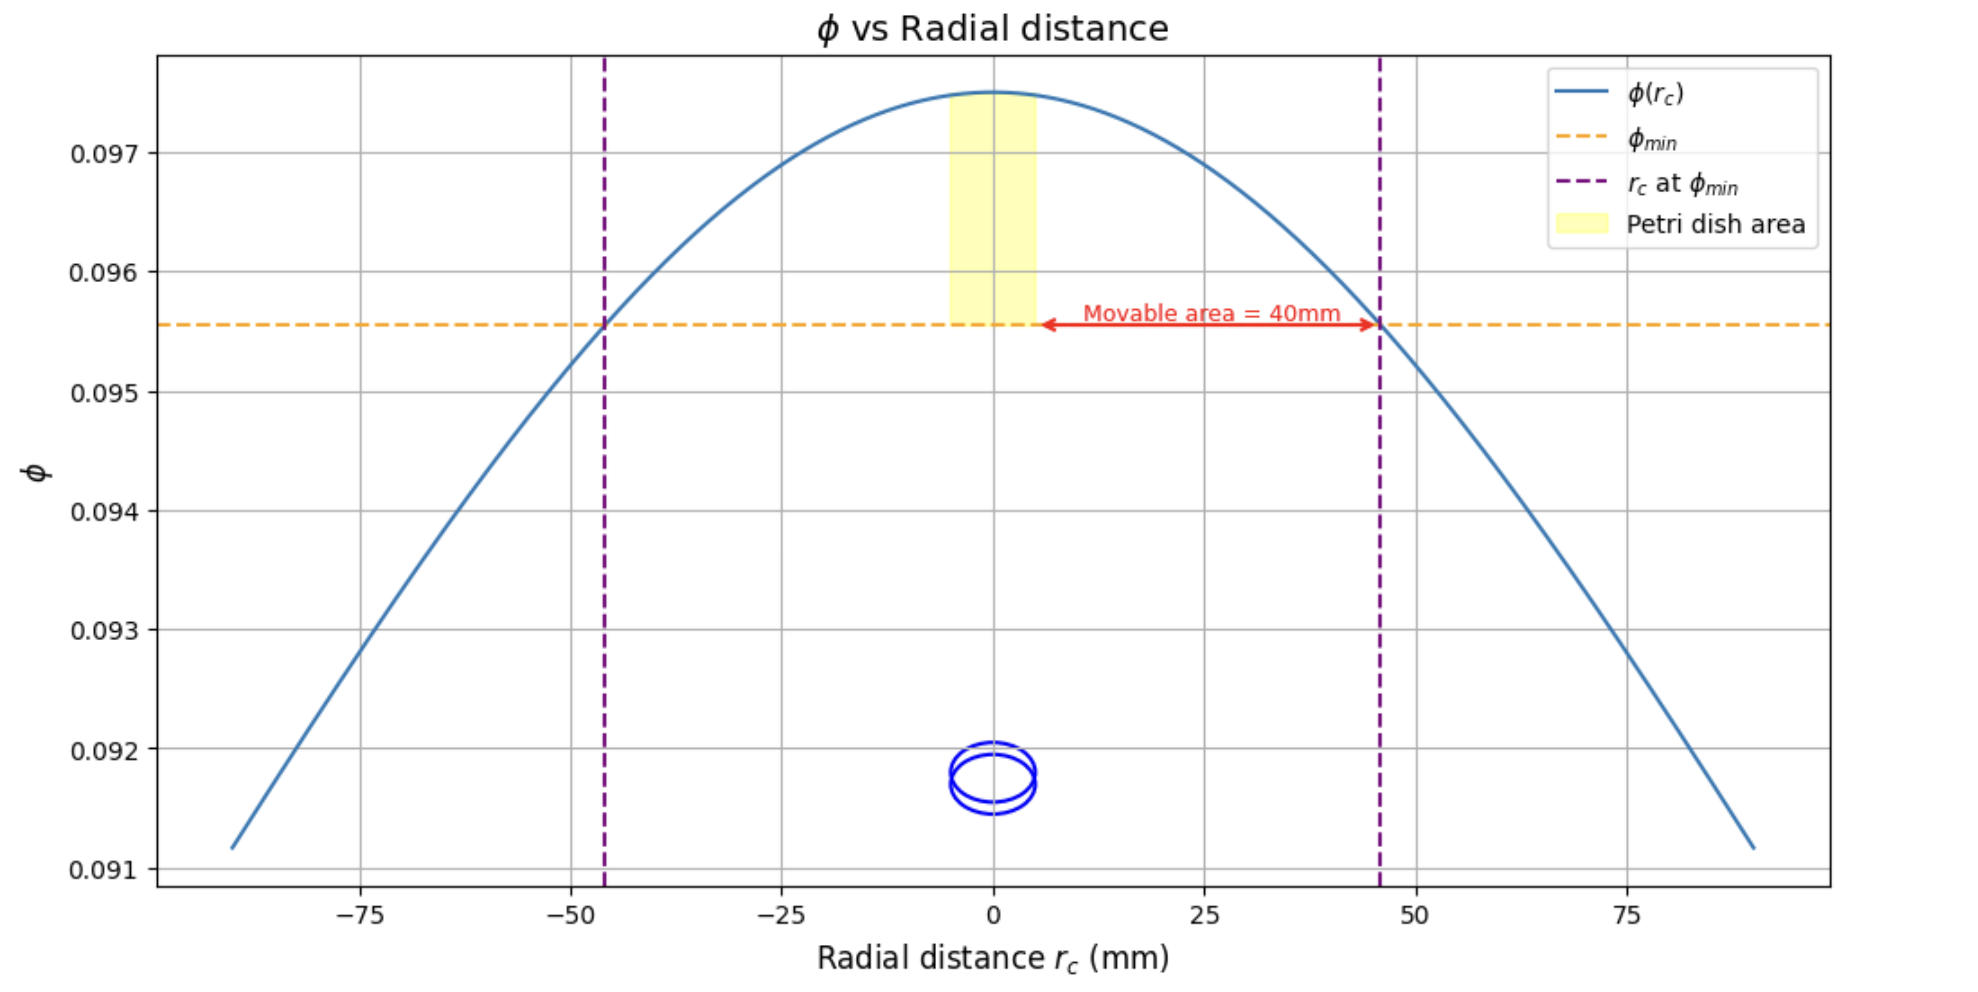
\includegraphics[width=\textwidth]{images/Screenshot 2024-03-22 at 09.42.18.png}
    \caption{The graph illustrates the illumination intensity (\( \phi \)) as a function of radial distance from the center of a Petri dish, represented by an oval at the bottom center. The shaded area within \(\pm 10\,mm\) indicates the physical size of the Petri dish. A movable area of approximately 40.87 mm from the edge of the Petri dish to the radial distance corresponding to \( \phi_{\min} \) is highlighted, demonstrating the operational range within which the chemical diode effectively inhibits the reaction. Beyond this range, the diode becomes non-operational, allowing the reaction to proceed unimpeded.}
    \label{fig:petri-dish-illumination}
\end{figure}

In this analysis, \( \phi_{\text{passive}} \) is defined as the maximum illumination intensity under which the Belousov-Zhabotinsky (BZ) reaction-based chemical diode remains in a passive state, effectively inhibiting the chemical reaction from propagating. The diode operates within this passive state until the illumination intensity decreases to a critical threshold, \( \phi_{\min} = 0.09555 \). Below this threshold, the diode becomes non-operational and ceases to inhibit the reaction, allowing it to propagate freely. The state of no light, denoted as \( \phi_{\text{active}} \), represents an ideal condition that is not physically achieved in this setup but is simulated using a filter to create the circuit pattern. \( \phi_{\min} \) was chosen based on experimental configurations and literature by Gorecki et al., signifying the operational limit for the diode's passive behavior. This analysis emphasizes the transition from \( \phi_{\text{passive}} \) to a non-operational state as light intensity falls below \( \phi_{\min} \), underscoring the critical operational range for the chemical diode's function in the BZ reaction.

Given the results shown in graph \ref{fig:petri-dish-illumination}, the maximum size of the Petri dish for a chemical diode is approximately 
Given the Petri dish size of 10 mm and extending 35.87 mm in both directions, the maximum chemical circuit size, considering the limitations of \( \phi_{\text{min}} \) and \( \phi_{\text{max}} \), can be calculated as:

\[ \text{Maximum Circuit Size} = 10\,mm + 40.87\,mm + 40.87\,mm = 91.74\,mm \]


\section{Light Impact on a CMM Neural Network \citep{stovold2017reaction}} \label{sec:light-impact-cmm-neuron}

A CMM neuron is an example of a larger chemical circuit. It is going to serve as an example project for applying the limits found in the previous section.
First we need to find the size of the curcuit in pixels as reported by \cite{stovold2017reaction}. In the paper the 
size of the whole computer is reported as \textbf{1998x646px} and uses the exact same configuration as covered in Table \ref{tab:simulation-parameters} in Chapter \ref{ch:design-implementation}.

Using the mapping established in Section \ref{sec:mapping-simulation-to-real-life}, we can calculate the real-life size of the chemical computer.


Given the dimensions of the circuit in the simulation as $1998 \times 646$ pixels and the established scaling factor of $5 \, \text{px/mm}$, we can calculate the real-life dimensions of the circuit.  

The width and height in real life can be calculated as follows:

\begin{align*}
    \text{Width in millimeters} &= \frac{\text{Width in pixels}}{\text{Scaling factor}} = \frac{1998 \, \text{px}}{5 \, \text{px/mm}} = 399.6 \, \text{mm}, \\
    \text{Height in millimeters} &= \frac{\text{Height in pixels}}{\text{Scaling factor}} = \frac{646 \, \text{px}}{5 \, \text{px/mm}} = 129.2 \, \text{mm}.
\end{align*}
    
Therefore, the real-life dimensions of the circuit are $399.6 \, \text{mm} \times 129.2 \, \text{mm}$, which corresponds to the minimum size of a petri dish that can accommodate the CMM Neural Network.

Given that the maximum size of the Petri dish for the assumptions in \ref{ass:assumptions-light-intensity} and \ref{ass:assumptions-light-intensity-calculation} is 91.74mm, the CMM Neural Network is too big to 
have its diode ciruits operate within the operational range of the chemical diode. 
The limits established are minimal limits/soft limits, meaning that the chemical computer in \cite{stovold2017reaction} uses much more than diodes and 
likely has tighter constraints, so if it cannot work under even the minimal limits, it is not going to work under the tighter constraints. 
    

\section{Light Impact on a single CMM Neuron \citep{stovold2017reaction}} \label{sec:light-impact-cmm-neuron-single}

We established that the big chemical computer in \cite{stovold2017reaction} is not possible under the conditions and assumptions established in the previous sections.
However, will a single neuron be possible? 
The size of a single CMM neuron from the paper is not specified, but there is only a design that mentions $200 \times 145$ pixels, however it is 
obvious from the images of the network that the neuron used is smaller and more compact than the designed one. This is why we are going to build a similar neuron
and measure it, which is done in Figure \ref{fig:neuron-cell-built}.
To calculate the size of the neuron as described by \cite{stovold2017reaction}, we begin by building a neuron cell 
that has similar dimentions to the one in the original paper.

\begin{figure}[h]
    \centering
    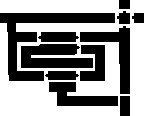
\includegraphics[width=0.75\textwidth]{images/circuit2-Recovered.png}
    \caption{Image of a single neuron cell sized at 116x144px built and tested in our simulation, which will be used as a reference for scaling to the approximate size of a single neuron in \cite{stovold2017reaction}.}
    \label{fig:neuron-cell-built}
\end{figure}


The width and height of the neuron in millimeters can be calculated as follows:

\begin{align*}
\text{Width in millimeters} &= \frac{\text{Width in pixels}}{\text{Scaling factor}} = \frac{116 \, \text{px}}{5 \, \text{px/mm}} = 23.2 \, \text{mm}, \\
\text{Height in millimeters} &= \frac{\text{Height in pixels}}{\text{Scaling factor}} = \frac{144 \, \text{px}}{5 \, \text{px/mm}} = 28.8 \, \text{mm}.
\end{align*}

Thus, the real-life dimensions of a single neuron, as adapted from the simulation, are $23.2 \, \text{mm} \times 28.8 \, \text{mm}$ and are well within the operational range for a chemical diode. 
However, the assumptions here might not be adequate as the neuron in the paper is likely to have tighter constraints than the chemical diode because it also uses a coincidence detector (AND gate),
a cross-junction with diodes that might have different constraints than a single diode due to its compact size and potentially other smaller details that might contribute to 
shrinking constraints. This is covered in Section \ref{sec:other-components}.



Also, even if the neuron cell might work under some conditions, that does not mean that it would function correctly as a whole computer because 
the change in illumination affects propagation times \citep{reddy1995effect} as seen in Section \ref{sec:light-imperfections}.
Chemical computers have no clock signal and rely heavily on correct signal arrival, so larger circuits like \cite{StovoldJames2019RaGI} 
might be heavily affected as they rely on propagation to ensure proper arrival of information.

\subsection{Testing the Custom CMM Neuron with different values of $I_p$}\label{sec:testing-neuron}
Manual tests with different $\phi_{\text{passive}}$ values have revealed that the neuron cell is operational at \( I_p \geq 0.99 \), which means the constraints for the operation are indeed very tight.
This is likely due to the AND gate operating under tighter constraints and the compactness of the neuron. 

In conclusion it is unclear if the neuron cell can be recreated in the real environment and more investigation is needed.

